\subsection{The cost of a screen with the Jev-like network does not grow with the number of pockets}

The dual encoder embeds every ligand once, and the scoring of a pocket is a matrix product. A joint network pays its interaction layers for every ligand-pocket pair. Table~\ref{tab:cost} and Figure~\ref{fig:cost}a give the time to screen all \tmALig{} ligands of DOCKSTRING from SMILES to scores on one \tmAGpu{}, measured at the full scale. The dual encoder needs \tmADualFiftySevenFull{} s for 57 pockets and \tmADualThousandFull{} s for 1{,}000 pockets, of which \tmAFeat{} s is the featurization of the ligands on the CPU. One more pocket adds \tmADualPerPocketMs{} ms to its model time. The cross-attention network needs \tmAXaHalfFiftySevenFull{} s in float16 and \tmAXaSingleFiftySevenFull{} s in float32 for 57 pockets, and \tmAXaHalfThousandFull{} and \tmAXaSingleThousandFull{} s for 1{,}000 pockets. One more pocket adds \tmAXaHalfPerPocket{} s in float16 and \tmAXaSinglePerPocket{} s in float32. The cross-attention network therefore needs \tmARatioXaHalfFiftySevenFull{} to \tmARatioXaSingleFiftySevenFull{} times the time of the dual encoder for 57 pockets and \tmARatioXaHalfThousandFull{} to \tmARatioXaSingleThousandFull{} times for 1{,}000 pockets. Without the featurization, which every network needs, the ratios of the model times are \tmARatioXaHalfFiftySevenModel{} to \tmARatioXaSingleFiftySevenModel{} for 57 pockets and \tmARatioXaHalfThousandModel{} to \tmARatioXaSingleThousandModel{} for 1{,}000 pockets (Supporting Information).

Uni-Dock docks \dockRateFastest{} ligands per second in its fastest search mode, which puts the \pocketPairs{} million pairs of the library against 57 pockets at \pocketDockDaysFast{} GPU-days. The dual encoder ranks the same pairs in \tmADualFiftySevenFull{} s. The time of the networks includes the featurization of the ligands from SMILES, and the time of the docking leaves out the preparation of the ligand files. Figure~\ref{fig:cost}b puts recall and time together. For 1{,}000 pockets the dual encoder has a recall of \kfDualTen{} at \tmADualThousandFull{} s and the cross-attention network a recall of \kfXattnTen{} at \tmAXaHalfThousandFull{} s in float16.

\begin{figure*}[t]
\centering
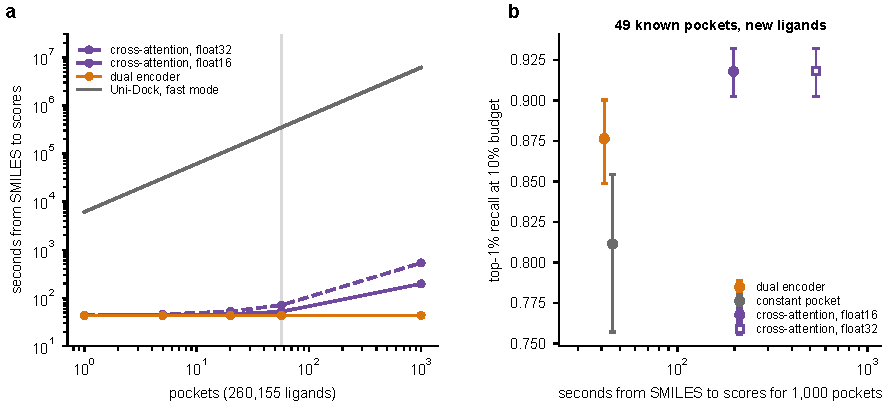
\includegraphics[width=\linewidth]{figures/fig_cost}
\caption{Cost and recall of the Jev-like and the joint network. (a) Time from SMILES to scores to screen the \tmALig{} ligands of DOCKSTRING against $P$ pockets on one \tmAGpu{}, measured at the full scale (markers), and the time of Uni-Dock in its fastest search mode (line). The vertical line marks the 57 pockets of DOCKSTRING, and the 1{,}000 pockets use them cyclically. (b) Top-1\% recall at the 10\% budget on the \kfNTargets{} known pockets for ligands that were not used in training (95\% intervals over the pockets) against the time for 1{,}000 pockets. The constant pocket is the dual encoder trained with one dummy pocket.}
\label{fig:cost}
\end{figure*}

\begin{table}[t]
\caption{Time to screen the 260{,}155 ligands of DOCKSTRING from SMILES to scores at the full scale on one RTX 4090 (seconds; best of two runs for the GPU stages, featurization of the SMILES on 32 CPU processes included). 1{,}000 pockets are the 57 pockets of DOCKSTRING used cyclically. Uni-Dock: library size times the number of pockets divided by the median docking rate of the fast mode at 4{,}000 ligands per call, without ligand preparation. The model time and every stage are in the Supporting Information.}
\label{tab:cost}
\centering
\footnotesize
\setlength{\tabcolsep}{4pt}
\begin{tabular}{lrr}
\toprule
Network & 57 pockets & 1{,}000 pockets \\
\midrule
Dual encoder & 43.3 & 43.5 \\
Cross-attention, float16 & 52.0 & 197 \\
Cross-attention, float32 & 71.1 & 535 \\
Uni-Dock, fast mode & 349{,}204 & 6{,}126{,}390 \\
\bottomrule
\end{tabular}
\end{table}

